\documentclass[crop,tikz]{standalone}% 'crop' is the default for v1.0, before it was 'preview'
%\usetikzlibrary{...}% tikz package already loaded by 'tikz' option
\begin{document}
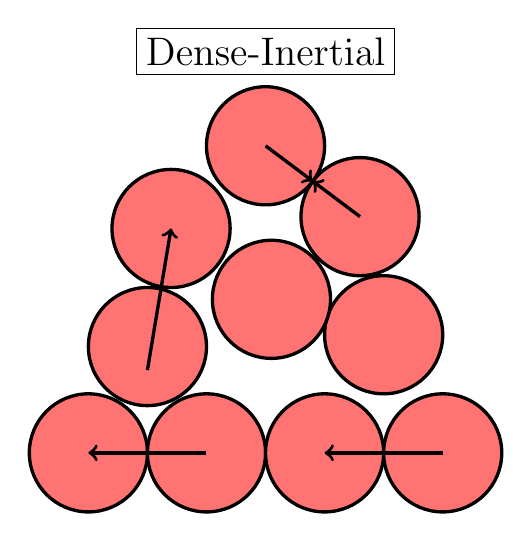
\begin{tikzpicture}[scale = 1.5]
    % \draw (-11.5,4) node {\textbf{A}};
    % \draw (-1.5,4) node {\textbf{B}};

    \def \b {-7};
    \def \c {0.1};
    \def \d {0.1};
    \def \r {2.3};

    % \draw[color=black, fill=red!55, very thick] (-5, -3.7) circle (1);
    % \draw[color=black, fill=red!55, very thick] (-5 + 1.42, 1.42-3.7) circle (1);
    % \draw[->, very thick] (0-5, 0-3.7) -- (0.72-5, 0.72-3.7) ;
    % \draw[->, very thick] (1.42-5, 1.42-3.7) -- (0.72-5, 0.72-3.7 );

    \node[draw] at  (-4.5, 3.7) { \Large Dense-Inertial};
    % \node[draw] at (-4,2.7-3.7) { \Large Collision};

    \foreach \x in {1, ..., 4}
            \draw [color=black, fill=red!55,very thick] (\x + \b, 0.3) circle (0.5);

    % \foreach \x in {1.5, ..., 3.5}
    %         \draw [color=black, fill=red!55, very thick] (\x + \b, 1.3) circle (0.5);
            
    \draw [color=black, fill=red!55, very thick] (1.5 + \b, 1.2) circle (0.5);       
    \draw [color=black, fill=red!55, very thick] (3.5 + \b, 1.3) circle (0.5);  
    \draw [color=black, fill=red!55, very thick] (2.55 + \b, 1.6) circle (0.5);
    \draw [color=black, fill=red!55, very thick] (3.3 + \b, 2.3) circle (0.5);
    \draw [color=black, fill=red!55, very thick] (1.7 + \b, 2.2) circle (0.5);
    \draw [color=black, fill=red!55, very thick] (2.5 + \b, 2.9) circle (0.5);


        
    \draw [very thick, ->] (2.5 + \b, 2.9) -- (2.9 + \b, 2.6);
    \draw [very thick, ->] (3.3 + \b, 2.3) -- (2.9 + \b, 2.6);
    
   \draw [very thick, ->] (1.5 + \b, 1.) -- (1.7 + \b, 2.2);

    \draw [very thick, ->] (2. + \b, 0.3) -- ( 2.+ \b -1  , 0.3);
    \draw [very thick, ->] (4. + \b, 0.3) -- ( 4.+ \b -1  , 0.3);

    
\end{tikzpicture}
\end{document}